\documentclass[a4paper,10pt]{article}

\usepackage[latin1]{inputenc}
\usepackage[T1]{fontenc}
\usepackage{lmodern}
\usepackage{times}

\usepackage[american]{babel}
\usepackage{ae,aecompl}
\usepackage{graphicx}

\usepackage[hang,bf,sf]{subfigure}
\subfigcapmargin=1em

\usepackage[plainpages=false,pdfpagelabels]{hyperref}

\usepackage{html}

\usepackage[round]{natbib}
\usepackage{amsmath}
\usepackage{amsfonts}
\usepackage{listings}
\newcommand*{\mynewline}{\def\space{ }\reflectbox{\ding{229}}}
\newcommand{\MyHookSign}{\hbox{\ensuremath\hookleftarrow}}
\lstset{escapechar=\%, frame=tb, basicstyle=\footnotesize, breaklines=true, prebreak={\MyHookSign}, showstringspaces=false, breakatwhitespace=true}
% 

\usepackage[margin=0.5cm,indention=-3em,font=small,labelfont={bf,sf},format=hang]{caption}

\usepackage{rotating}
\usepackage{longtable}
\usepackage{multirow}
\usepackage{color}
\usepackage{colortbl}
\usepackage{booktabs}
\usepackage[automark]{scrpage2}
\pagestyle{scrheadings}
\chead{}
\cfoot{}
\lehead{\headmark}
\rohead{\headmark}
\lefoot{\hrule\pagemark}
\rofoot{\hrule\pagemark}

% Keine "Schusterjungen"
\clubpenalty = 10000
% Keine "Hurenkinder"
\widowpenalty = 10000  \displaywidowpenalty = 10000
% �berstehende Zeilen vermeiden 
\tolerance=9000

\newcommand{\filename}[1]{\textit{\texttt{\small #1}}}
\newcommand{\opname}[1]{\textit{\texttt{\small #1}}}
\newcommand{\opnamesmaller}[1]{\textit{\texttt{\scriptsize #1}}}
\newcommand{\JPetStore}[0]{\textsf{JPetStore}}

\newcommand{\JakartaJMeter}[0]{\textsf{Apache JMeter}}
\newcommand{\ApacheJMeter}[0]{\textsf{Apache JMeter}}
\newcommand{\JMeter}[0]{\textsf{JMeter}}

\newcommand{\MarkovForJMeter}[0]{\textsf{Markov4JMeter}}
\newcommand{\MarkovState}[0]{\textsf{Markov State}}
\newcommand{\MarkovStates}[0]{\textsf{Markov States}}
\newcommand{\MarkovSessionController}[0]{\textsf{Markov Session Controller}}
\newcommand{\MarkovSessionControllers}[0]{\textsf{Markov Session Controllers}}
\newcommand{\SessionArrivalController}[0]{\textsf{Session Arrival Controller}}
\newcommand{\BehaviorMixController}[0]{\textsf{Behavior Mix Controller}}
\newcommand{\BehaviorModels}[0]{behavior models}
\newcommand{\BehaviorModel}[0]{behavior model}
\newcommand{\BehaviorMix}[0]{behavior mix}

%opening
\title{\MarkovForJMeter{} Tutorial}
\author{Andr\'{e} van Hoorn}

\begin{document}

\maketitle

\begin{abstract}

\end{abstract}

By extending \htmladdnormallink{\ApacheJMeter{}}{http://jakarta.apache.org/jmeter/} with \MarkovForJMeter{} you're able to execute \textit{Test Plans} based on configurable probabilistic \BehaviorModels{}: given a currently visited Web site, the next site to be requested is chosen based on configurable probability values. Moreover, \MarkovForJMeter{} allows to define how to vary the number of active user threads during test execution.

Our paper describing the the probabilistic and intensity-varying workload generation approach has been published in the proceedings of the \textit{SPEC International Performance Evaluation Workshop 2008 (SIPEW '08)}:

\begin{quotation}\small\sffamily
Andr\'e~van Hoorn, Matthias~Rohr, and Wilhelm~Hasselbring. \htmladdnormallink{\emph{Generating Probabilistic and Intensity-varying Workload for Web-based Software Systems}}{http://trustsoft.uni-oldenburg.de/Members/andrevh\#vanHoornRohrHasselbring2008GeneratingProbabilisticAndIntensityVaryingWorkloadForWebBasedSoftwareSystems}. In Performance Evaluation -- Metrics, Models and Benchmarks: Proceedings of the SPEC International Performance Evaluation Workshop (SIPEW '08), vol. 5119 of
  \emph{Lecture Notes in Computer Science (LNCS)}, pages 124--143. Heidelberg: Springer (June 2008).
\end{quotation}

Throughout this tutorial, we will give installation instructions and show how to create an executable \textit{Test Plan} for the \htmladdnormallink{iBATIS}{http://ibatis.apache.org/} \JPetStore{} sample application. The JMX file of the Test Plan and the associated files can be found in the directory \filename{examples/jpetstore/tutorial} of the \MarkovForJMeter{} release. Extended example JMX file which are not covered by this tutorial are included as well.

We assume that you installed \ApacheJMeter{} version 2.2 or higher %\citep{JMeter}
and know how to use it. \MarkovForJMeter{} requires the Java Runtime Environment versioned 1.5 or higher. %\citep{Sun2007}

\section{Downloading and Installing \MarkovForJMeter{}}

From the \MarkovForJMeter{} homepage \url{http://markov4jmeter.sourceforge.net} you can download  %\citep{Hoorn2007}
 two types of archives:

\begin{description}
 \item [Source Archives:]
The source archive contains the \MarkovForJMeter{} sources. These archive names follow the pattern \filename{markov4jmeter-\-<version>\-\_src.\{zip|tgz\}}. This archive is required when \MarkovForJMeter{} shall be modified and compiled. It includes further instructions to do so.

 \item [Runtime Archives:]
The runtime archive contains a runnable version of \MarkovForJMeter{} which can be used with \JMeter{}. These archive names follow the pattern \filename{markov4jmeter-\-<version>.\{zip|tgz\}}. 
\end{description}

\noindent In order to install a runnable version of \MarkovForJMeter{}, the following steps need to be performed:

\begin{enumerate}
\item Download and extract the \MarkovForJMeter{} runtime archive in the desired file type (tgz- or zip-format). 
\item Copy the \filename{Markov4JMeter.jar}, which resides inside the \filename{dist/} directory, to the directory \filename{lib/ext/} of the \JMeter{} installation.
\item After restarting \JMeter{}, two new entries within the Logic Controllers menu exist: \MarkovState{} and \MarkovSessionController{} (see Figure~\ref{fig:markovForJMeter:newControllerMenuAppendix}).\\

\begin{figure}[h!]
 \centering
 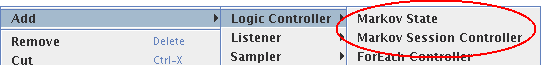
\includegraphics[width=0.75\textwidth]{figures/markov4jmeter_newControllerMenu_highlighted.png}
 % markov4jmeter_newControllerMenu.png: 650x100 pixel, 173dpi, 9.54x1.47 cm, bb=0 0 271 42
 \caption[New entries in context menu]{After installing \MarkovForJMeter{}, the Logic Controller menu shows two new entries: \MarkovState{} and \MarkovSessionController{}.}
 \label{fig:markovForJMeter:newControllerMenuAppendix}
\end{figure}
\end{enumerate}

\section{Using \MarkovForJMeter{}}

This section contains a step-by-step description how a simple probabilistic Test Plan for the \JPetStore{} is created. We use the publicly accessable \JPetStore{} instance hosted by \url{http://www.jwebhosting.net/}, such that you're not required to set up your own \JPetStore{} in order just to follow the instructions given in this tutorial. Hence, please keep the number of parallel users emulated by your first \MarkovForJMeter{} experiments small in order not to cause too much load on the provided server. A \MarkovForJMeter{} Test Plan can then be executed just like any ordinary \JMeter{} Test Plan. 

\subsection*{Preparing the Test Plan}

By performing the following steps, the basic Test Plan shown in the left-hand side of Figure~\ref{fig:markov4jmeter:preparedTestPlan} is created.

\begin{enumerate}
\addtolength{\itemsep}{-10pt}
 \item Add a \textit{Thread Group} to the empty \textit{Test Plan} and select to stop the test when a sampler error occurs. Set the number of threads to $5$ and the loop count to $5$ without using the \textit{Scheduler}.
 \item Add an \textit{HTTP Cookie Manager} from the \textit{Config Element} menu to the \textit{Thread Group} and select the cookies to be deleted after each iteration.
 \item Add the \textit{HTTP Request Defaults} from the \textit{Config Element} menu and insert the data shown in Figure~\ref{fig:markov4jmeter:preparedTestPlan}.
 \item Add a \textit{View Results Tree} for debugging purposes and select ``Save Response Data''.
\end{enumerate}

\begin{figure}[h!]
 \centering
 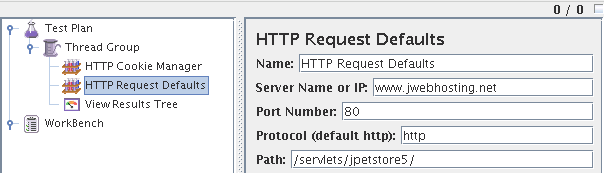
\includegraphics[width=\textwidth]{figures/markov4jmeter_preparedTestPlan.png}
 % markov4jmeter_preparedTestPlan.png: 604x174 pixel, 85dpi, 18.05x5.20 cm, bb=0 0 512 147
 \caption[Prepared JMeter Test Plan]{A prepared \JMeter{} Test Plan.}
 \label{fig:markov4jmeter:preparedTestPlan}
\end{figure}

\subsection*{Adding a Markov Session Controller}%\label{sec:tutorial:addSessionCtrl}

\begin{figure}
 \centering
 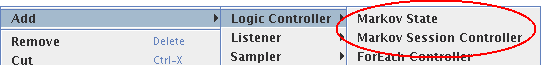
\includegraphics[width=0.75\textwidth]{figures/markov4jmeter_newControllerMenu_highlighted.png}
 % markov4jmeter_newControllerMenu.png: 650x100 pixel, 173dpi, 9.54x1.47 cm, bb=0 0 271 42
 \caption[New entries in context menu]{After installing \MarkovForJMeter{}, the Logic Controller menu shows two new entries: \MarkovState{} and \MarkovSessionController{}.}
 \label{fig:markovForJMeter:newControllerMenuMain}
\end{figure}

After installing \MarkovForJMeter{}, the new Logic Controllers \MarkovState{} and \MarkovSessionController{} appear in the respective menu (see Figure~\ref{fig:markovForJMeter:newControllerMenuMain}).

A \MarkovSessionController{} needs to be added to the \textit{Thread Group}. This is the root element of any probabilistic session model consisting of a number of \MarkovStates{} and transitions between them. Also, it contains the configuration of the \BehaviorMix{} and the \SessionArrivalController{}. A \textit{Gaussian Random Timer} added to the \MarkovSessionController{} emulates client-side think times between subsequent requests.

It is highly recommended to use at most one \MarkovSessionController{} within a Test Plan. The \MarkovSessionController{} should be placed at the root level of the Thread Group. Especially, \MarkovSessionControllers{} must not be nested.

\subsection*{Adding  Markov States}%\label{sec:tutorial:addMarkovStates}

\begin{table}
\small
\sffamily
\centering
% use packages: array
\scalebox{0.8}{
\sffamily
\begin{tabular}{|ll|l|l|l|l|}
\hline
&\textbf{Name} & \textbf{Path} & \textbf{Method} & \multicolumn{2}{c|}{\textbf{Parameters}} \\
& &  &  & Name & Value \\ \hline\hline
\multicolumn{6}{|l|}{\textbf{Markov State}: Index}\\ \hline
& index.shtml & [JPSROOT]/index.shtml & GET & &\\\hline
\multicolumn{6}{|l|}{\textbf{Markov State}: Sign On}\\ \hline
& signonForm.shtml & [JPSROOT]/signonForm.shtml & GET & &\\ \hline
& signon.shtml & [JPSROOT]/signon.shtml & POST & username & j2ee \\
&  & & & password & j2ee\\
&  & & & submit & Login\\ \hline
\multicolumn{6}{|l|}{\textbf{Markov State}: View Category}\\ \hline
& viewCategory.shtml & [JPSROOT]/viewCategory.shtml & GET & categoryId & REPTILES\\ \hline
\multicolumn{6}{|l|}{\textbf{Markov State}: Sign Off} \\ \hline
& signoff.shtml & [JPSROOT]/signoff.shtml & GET &  &\\ \hline
\end{tabular}}
\caption[Configuration of HTTP Request Samplers]{Data to fill in to the \textit{HTTP Request} configuration dialogs. ``[JPSROOT]'' needs to be replaced with ``/servlets/jpetstore5/shop''. Also, the check boxes ``Redirect Automatically'' and ``Follow Redirects'' must be selected.}
\label{tbl:markov4jmeter:httpRequestDetails}
 
\end{table}

After adding four  \MarkovStates{} named ``Index'', ``Sign On'', ``View Category'', and ``Sign Off'' to the \MarkovSessionController{}, the Test Plan has the tree structure shown in Figure~\ref{fig:markov4jmeter:testplan}. \MarkovStates{} must be placed directly underneath a \MarkovSessionController{} and must especially not be nested -- neither directly nor indirectly. Each \MarkovState{} must have a unique name. \textit{HTTP Request Samplers} should be added to the \MarkovStates{} according to Table~\ref{tbl:markov4jmeter:httpRequestDetails}.

\begin{figure}[h]
\centering
 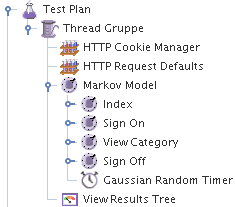
\includegraphics[width=0.35\textwidth]{figures/markov4jmeter_testPlan.png}
\caption[Markov4JMeter Test Plan]{\MarkovForJMeter{} Test Plan.}
\label{fig:markov4jmeter:testplan}
\end{figure}

\subsection*{Defining Transition Guards and Actions}%\label{sec:tutorial:defineTransitions}

When selecting a \MarkovState{} within the Test Plan, the configuration dialog including the table to define guards and actions for transitions to all states of the same \MarkovSessionController{} appears. The table is automatically updated each time \MarkovStates{} are added, removed or renamed. Transitions can be assigned \textit{guards} in order to allow a transition to be taken only if the specified expression evaluates to \textit{true}. By selecting the respective check box, transitions can be deactivated completely, which is equivalent to entering a guard evaluating to \textit{false}. An \textit{action} is a list of statements, such as function calls or variable assignments, separated by a semicolon
% \footnote{See \url{http://jakarta.apache.org/jmeter/usermanual/functions.html} for an overview of functions already provided by \JMeter{}.} 
which is evaluated when a transition is taken. 

In our example a variable \textit{signedOn} is used to remember whether a user has logged in or not. A \textit{User Parameters Pre-Processor} to the \MarkovSessionController{} with a new variable named \textit{signedOn} with the value \textit{false} to initialize the variable. The check box ``Update Once Per Iteration'' needs to be activated. The guards and actions of the transitions should be configured as listed in Table~\ref{tbl:markov4jmeter:transitions}.

\begin{table}[h]
\small
\sffamily
\centering
% use packages: array
%\scalebox{0.8}{
\begin{tabular}{|l|l|l|l|l|}
\hline
\textbf{Source State} & \textbf{Destination State} & \textbf{Disabled} & \textbf{Guard} & \textbf{Action} \\ \hline\hline
\textit{any} & Sign On &  & !\$\{signedOn\} & signedOn=true\\\hline
\textit{any} & Sign Off & & \$\{signedOn\}  & signedOn=false\\\hline
\end{tabular}
\caption[Configuration of guards and actions]{Guards and actions used to restrict transitions to the states ``Sign On'' and ``Sign Off''. The variable \textit{signedOn} is used to remember whether a user has logged in or not.}
\label{tbl:markov4jmeter:transitions}
%}
\end{table}

\subsection*{Creating User Behavior Models and Defining the BehaviorMix}%\label{sec:tutorial:createBehaviorModel}

A behavior file template can be exported by clicking the button ``Generate Template'' within the \MarkovSessionController{}. This file can then be edited in a spread sheet application or a text editor. The sum of probabilities in each row must be $1.0$. This step needs to be performed for each \BehaviorModel{} to be used. 

The \BehaviorMix{}, i.e. the assignment of \BehaviorModels{} to their relative frequency of occurrence during execution, is defined in the configuration dialog of the \MarkovSessionController{}. Entries can be added and removed using the buttons ``Add'' and ``Delete''. Again, the sum of relative frequencies must be $1.0$. Absolute and relative filenames can be used. Relative filenames are always relative to the directory \JMeter{} has been started from. Figure~\ref{fig:markov4jmeter:behaviorMix} shows an example behavior mix.

\begin{figure}[h]
 \centering
 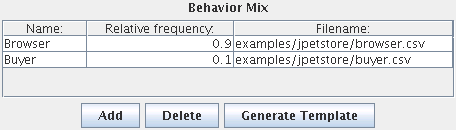
\includegraphics[width=0.6\textwidth]{figures/markov4jmeter_behaviorMix.png}
 % markov4jmeter_behaviorMix.png: 456x130 pixel, 85dpi, 13.63x3.89 cm, bb=0 0 386 110
 \caption{Example Behavior Mix.}
 \label{fig:markov4jmeter:behaviorMix}
\end{figure}

\noindent If an error occurs while loading the \BehaviorModels{}, the entire test is aborted immediately. Details concerning this error are written to the file \filename{jmeter.log}.

\subsection*{Using the Session Arrival Controller}%\label{sec:tutorial:useSessionArrivalCtrl}

\begin{figure}
\begin{lstlisting}[language=Java]
import org.apache.jmeter.util.JMeterUtils;

long startMs = Long.parseLong(JMeterUtils.getPropDefault("TEST.START.MS",""));
long curMs = System.currentTimeMillis();
double expMin = (curMs-startMs)/(1000*60);
return (int)Math.ceil(allowedNum(expMin));
\end{lstlisting}
\caption[Example BeanShell script defining number of active sessions]{Example BeanShell script which returns the elapsed experiment minute as an integer using the \MarkovForJMeter{} variable \textit{TEST.START.MS}.}
\label{fig:markov4jmeter:arrivalFormular}
\end{figure}

\noindent The \SessionArrivalController{} controls the number of active sessions, given an expression evaluating to an integer value. It is configured within the configuration dialog of the \MarkovSessionController{}. \JMeter{} allows to use BeanShell 
\footnote{Notice that the BeanShell Jar file is not included in the \JMeter{} release. The file can be downloaded from \url{http://www.beanshell.org/download.html} and must be copied to the \filename{lib/opt/} directory of the \JMeter{} installation. %See \url{http://www.beanshell.org/} to get an introduction to the BeanShell. 
See \url{http://jakarta.apache.org/jmeter/usermanual/functions.html\#__BeanShell} for a description on how to use BeanShell scripts within \JMeter{} expressions.} 
scripts within text expressions. Particularly, this allows for varying the number of active sessions depending on the elapsed experiment time. \MarkovForJMeter{} adds the global variable \textit{TEST.START.MS} to the \JMeter{} context which is accessible in BeanShell scripts. The variable is set when the Test Plan is started.

For example, when using the BeanShell script listed in Figure~\ref{fig:markov4jmeter:arrivalFormular}, the \SessionArrivalController{} limits the number of active sessions based on the elapsed experiment minute: in the $i$-th minute $i$ active sessions are allowed in parallel. Figure~\ref{fig:markov4jmeter:sessionArrivalProperties} shows how to use this BeanShell script within the \SessionArrivalController{} configuration.

\begin{figure}[h]
 \centering
 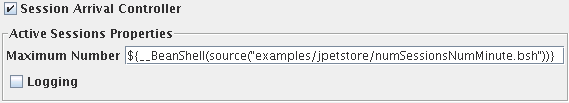
\includegraphics[width=0.8\textwidth]{figures/markov4jmeter_sessionArrivalProperties.png}
 % markov4jmeter_sessionArrivalProperties.png: 561x106 pixel, 85dpi, 16.77x3.17 cm, bb=0 0 475 90
 \caption[Using a BeanShell script within the Session Arrival Controller]{BeanShell scripts can be used with the function \textit{BeanShell}. The BeanShell function \textit{source} includes a script file.}
 \label{fig:markov4jmeter:sessionArrivalProperties}
\end{figure}

The \SessionArrivalController{} doesn't create any new threads. It simply blocks threads in a queue in case the number of active sessions would exceed the given maximum number. Hence, the maximum number of active sessions is limited to the number of threads configured in the \textit{Thread Group}.

If an error occurs while evaluating the active sessions formula, the entire test is aborted immediately. Details concerning this error are written to the file \filename{jmeter.log}.

\section{Running the Test}
 
Start the test run just as you would start any \JMeter{} test. You should always check \textit{jmeter.log} in order to get information about possible errors. You can use \JMeter{} to render the resulting HTML response data for each request in order to make sure you set up your Test Plan properly. 

\end{document}
